The purpose of this chapter is to benchmark and evaluate Memcached performance. Firstly, we will focus on Memcached performance ``out of the box''. Secondly, we will examine Memcached scalability in respect to threads which will provide us with an optimization baseline. It is worth noting that majority of Memcached user will end up using the default configuration, perhaps with increased threading level. Subsequently, we will explore the impact of assigning individual threads to CPU cores as well as the impact interrupt processing has on Memcached. Furthermore, we will explore a multi-instance setup as well as the impact object size has on Memcached performance. Finally, we will turn our attention to the distribution of cache keys.

Throughout this chapter, we will focus primarily on latency, 99th percentile latency and throughput. Where relevant, we will explore additional attributes. Unless otherwise stated, all performance tuning is done to meet a Quality of Service (QoS) constraint of 99th percentile latency under 1 millisecond.

\section{Shiny Fresh Memcached}
Firstly, let us focus on Memcached performance ``out of the box'', that is, Memcached with a default configuration. When we tear down the wrapping paper of a Memcached distribution, we are presented with two important configuration options - a) The port number memcached will listen on and b) the amount of memory we allocate to Memcached which determines the total capacity of the cache. For the purposes of this paper, we use port number 11120. The amount of memory we allocate to memcached is dependent on the total amount of memory available on the host machine as well as any additional workload on the host. In our case, we are the sole workload with a total of 8GB memory available to us. Throughout this paper, we choose to allocate 6 GB of memory to Memcached, leaving 2 GB for the operating system or remaining unused. Table \ref{tab:m_default_config} outlines the configuration options including relevant defaults. It is worth noting that in the default configuration Memcached runs with 4 threads.

\begin{table}[h!]
\centering
\begin{tabular}{| c c c |}
 \hline
 Configuration Option & Explanation & Value\\ [0.5ex]
 \hline\hline

 -d & Run in Daemon Mode & true \\
 -p & Port number & 11120 \\
 -t & Number of Threads & 4 (default) \\
 -m & Memory Allocated & 6144 (6GB) \\

 \hline

\end{tabular}
\caption{Memcached Configuration Options.}
\label{tab:m_default_config}
\end{table}

Given the configuration outlined in Table \ref{tab:m_default_config}, we can proceed and launch Memcached on the server with the following command:
\begin{lstlisting}
memcached -d -p 11120 -m 6144
\end{lstlisting}


Secondly, we configure the clients responsible for generating cache workload. In order to determine a saturation point of the serve cache, we increase the workload exerted by the clients linearly. Initially, we consider a workload provided by 3 threads and 1 connection per each workload generating server. Subsequently, the number of connections is increased linearly until a saturation point is found or QoS requirements are no longer satisfied. For the benchmark, and indeed for the rest of the paper unless otherwise stated, we consider an object size of 64 bytes. With object sizes of 64 bytes, we aim to generate a sufficiently large dataset in order to exceed the memory capacity provisioned for Memcached. In this case, we define the key space to be between 1 and 100 million, yielding a dataset 6.4GB large. Table \ref{tab:m_memtier_default} outlines the configuration options used.

\begin{table}[h!]
\centering
\begin{tabular}{| c c c |}
 \hline
 Configuration Option & Explanation & Value\\ [0.5ex]
 \hline\hline

 -s & Server & nsl200 (server hostname) \\
 -p & Port number & 11120 \\
 -c & Number of Connections & [1..10] \\
 -t & Number of Threads & 3 \\
 --key-minimum & Smallest key & 1 \\
 --key-maximum & Largest key & 100 000 000 \\
 --random-data & Generate Random Data & true \\
 --data-size & The size of data in bytes & 64 \\

 \hline

\end{tabular}
\caption{Memtier Configuration Options}
\label{tab:m_memtier_default}
\end{table}

The memtier\_benchmark (Memtier) can be launched with the following command:
\begin{lstlisting}
  memtier -s <server> -p 11120 -c <connections> -t 3
    --random-data
    --key-minimum=1
    --key-maximum=100000000
    --random-data
    --data-size=64
\end{lstlisting}

The application start commands are provided for clarity and will be omitted in subsequent benchmarks as they can be directly constructed from the configuration tables.

\subsection{Latency, Throughput and Number of Connections}

Firstly, we are interested in the relationship between throughput, latency and the number of connections. The relationship is shown in Figure \ref{fig:memcached-default-latency-vs-ops}. Latency, both mean and 99th percentile, are plotted on the left vertical axis, the number of operations per second is plotted on the right vertical axis and the number of connections used is on the horizontal axis.

\begin{figure}[h]
    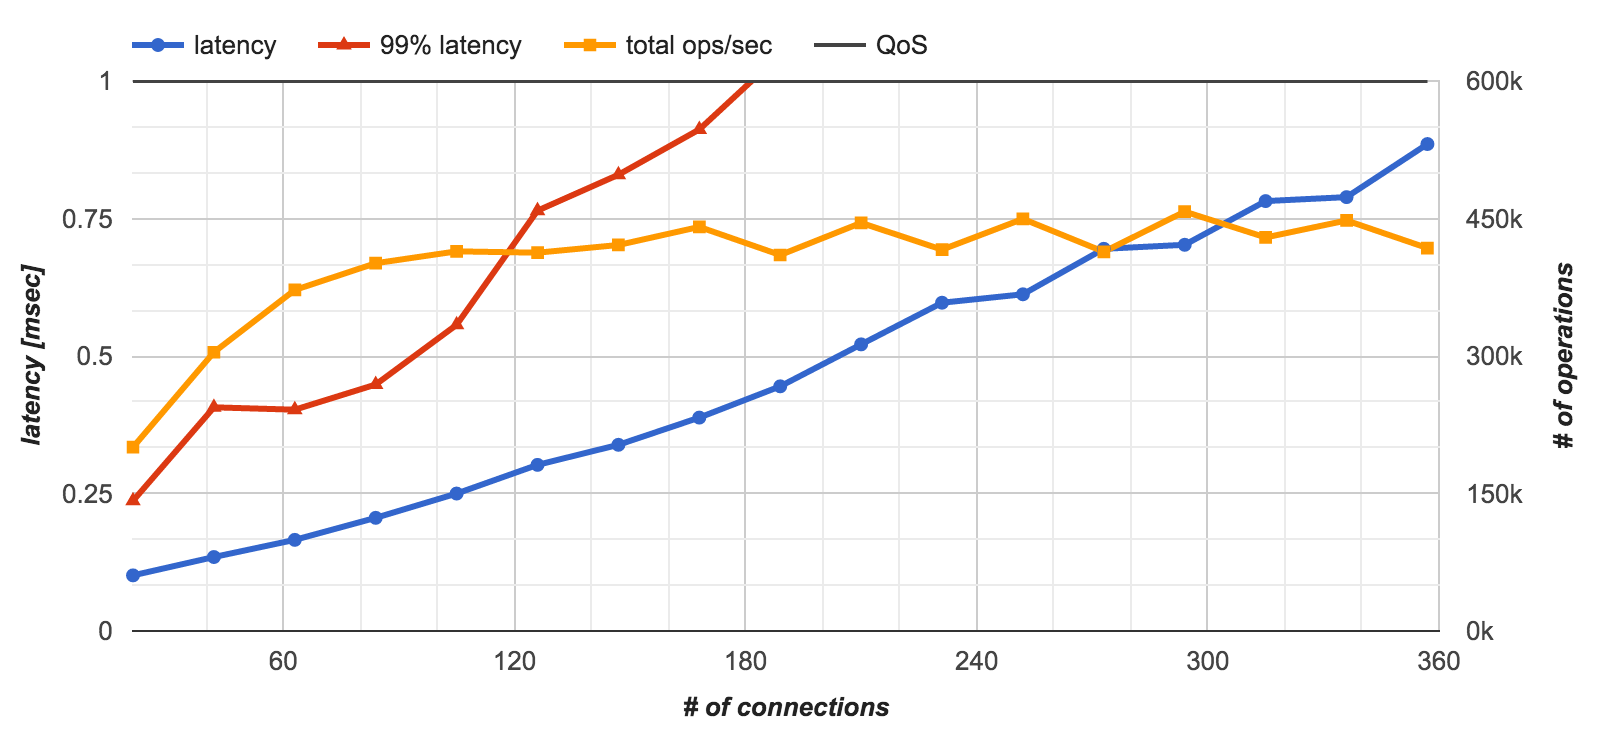
\includegraphics[width=\textwidth]{./res2/m_baseline_latency.png}
    \caption{Latency \& Throughput vs Number of Connections}
    \label{fig:memcached-default-latency-vs-ops}
\end{figure}

As the number of connection increases, so does mean latency. There is a linear relationship between the mean latency and the number of connections. This is an expected result, as the load increases linearly, we expect the mean latency to increase linearly too. An increase in the number of connections by 21 results in increased mean latency by approximately 0.09ms.

The 99th percentile latency increases linearly with the number of connections until we reach 105 connections. A further increase in the number of connections results in a disproportionately greater increase in tail latency. The maximum number of connections satisfying the QoS occurs at 147 connections and tail latency at 0.99ms. A further increase in load results in a steeper increase in tail latency. We can observe as the load increases, the tail latency diverges from the mean latency and increases at a faster pace.

The number of operations per second increases linearly with the number of connections and reaches a peak of 238k requests per second at 147 connections (within QoS). The total throughput appears to be largely unaffected by the steep increase in tail latency in this benchmark.


\subsection{CPU Utilization}

Secondly, we consider the effect of the workload on the Memcached server in terms of CPU Utilization. The CPU utilization is monitored through the \textit{mpstat} \cite{mpstat} utility which reports the percentage of CPU utilization broken down into multiple categories. The following table \cite{mpstat} summarizes the responsibilities of each category.

\begin{enumerate}
    \item [\%usr] Show the percentage of CPU utilization that occurred while executing at the user level (application).
    \item [\%sys] Show the percentage of CPU utilization that occurred while executing at the system level (kernel). Note that this does not include time spent servicing hardware and software interrupts.
    \item [\%iowait] Show the percentage of time that the CPU or CPUs were idle during which the system had an outstanding disk I/O request.
    \item [\%irq] Show the percentage of time spent by the CPU or CPUs to service hardware interrupts.
    \item [\%soft] Show the percentage of time spent by the CPU or CPUs to service software interrupts.
    \item [\%idle] Show the percentage of time that the CPU or CPUs were idle and the system did not have an outstanding disk I/O request.
\end{enumerate}

For the context of this paper, \textit{\%usr} corresponds directly to the CPU utilization used by Memcached as it is the only application running on the server.

Furthermore, \textit{\%soft} represents the software interrupt issued by \textit{libevent} when a new file descriptor is available for processing, that is, a new request is available to be processed or a response is ready to be handed over to the network stack.

\begin{figure}[h]
    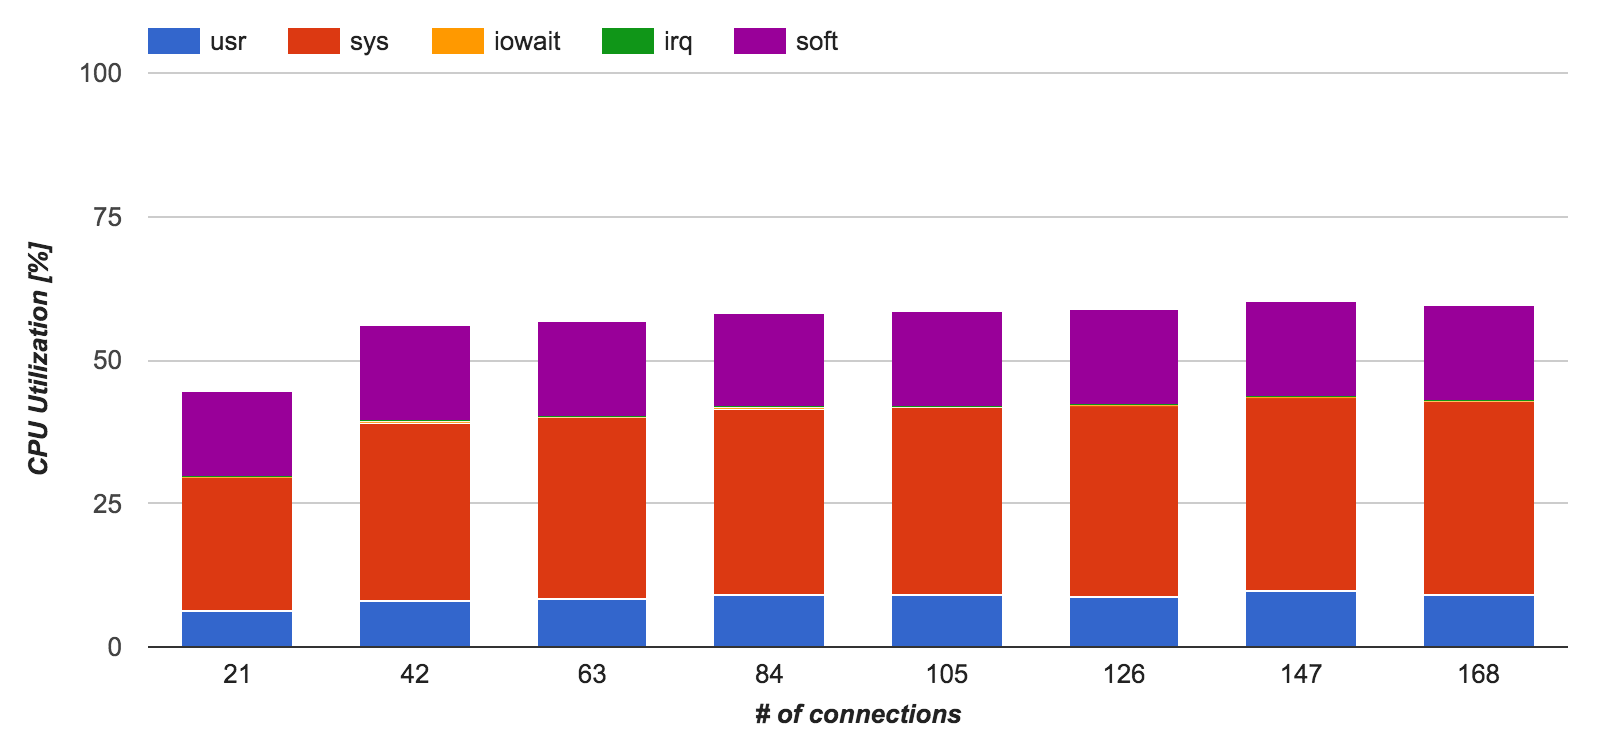
\includegraphics[width=\textwidth]{./res2/m_baseline_cpu.png}
    \caption{CPU Utilization for Out of the Box Configuration of Memcached}
    \label{fig:m_baseline_cpu}
\end{figure}

Figure \ref{fig:m_baseline_cpu} outlines the CPU Utilization broken down into mpstat categories. Note that unallocated percentage constitutes the \textit{idle} percentage of the CPUs.

Memcached utilization (\textit{usr}) increases slightly as the number of connections increases, however, overall remains stable and accounts for at most 9\% of the total utilization. The kernel (\textit{sys}) accounts for 33\%, a significant portion of the CPU utilization relative to other categories. The CPU utilization dedicated to processing software interrupts (\textit{soft}) accounts for 16\% of the total CPU utilization. This makes the second most significant category in the benchmark. Disk IO accounts for 0\% of total utilization as all data is stored in memory and we do not need to access the disk. Hardware interrupts (\textit{irq}) account for 0.01\% of total utilization.

Overall, CPU utilization starts at 48\% and increases to 60\% as the number of connections increases. We can observe that at this CPU utilization we have not been able to fully utilize the server resources. Additionally, the kernel and software interrupts account for majority of the total CPU utilization. This is indicative of a larger pattern of Memcached execution - Memcached performance is dominated by the kernel and network stack. This is consistent with findings in MICA \cite{lim2014mica}.


\subsection{Evaluation}
Given the trends presented in Figures \ref{fig:memcached-default-latency-vs-ops} and \ref{fig:m_baseline_cpu}, we can conclude the ``out of box'' configuration of Memcached does not deliver optimal performance. The number of operations per second could be increased by increasing CPU utilization which in turn  should result in improved tail latency. Additionally, we have been able to observe that the kernel and software interrupt performance dominates the CPU utilization. A simple approach to increasing CPU utilization is to increase the number of threads we provision for Memcached.

% ________________________________________________________

\section{Thread Scalability}
In this section, we focus on increasing CPU utilization through the use of multiple threads. We have shown that the default configuration results in underutilization of the server resources and argued that increased CPU utilization should result in improved performance. Memcached, as a high performance object cache, is designed to be executed on a multi-core architecture. Scalability is primarily implemented through the use of multi threading. It is worth noting that multi-threading also results in increased application complexity. Individual threads requiring access to shared data are required to obtain a lock before they can proceed with data manipulation. We design a benchmark which focuses on thread scalability by linearly increasing the number of threads Memcached is provisioned.

Empirically, we expect the best performance to be achieved when there are as many Memcached threads as there are CPU cores. The cache server is equipped with 6 CPU cores and therefore we would expect 6 threads to maximize performance. This is also suggested by Leverich and Kozyrakis \cite{leverich2014reconciling}. Utilizing less threads should result in underutilization of the CPU leading to sub-optimal throughput. More than 6 threads should conversely result in increased context switching overhead and therefore should lead to increased latency.

Utilizing results about the number of connections from previous section, we configure a constant level of workload with 3 Memtier threads and 7 connections per each thread. We maintain the same key-object configuration as in previous benchmark. The configuration details of the Memtier benchmark are outlined in Table \ref{tab:m_threads_memtier}.

\begin{table}[h!]
\centering
\begin{tabular}{| c c c |}
 \hline
 Configuration Option & Explanation & Value\\ [0.5ex]
 \hline\hline

 -s & Server & nsl200 (server hostname) \\
 -p & Port number & 11120 \\
 -c & Number of Connections & 7 \\
 -t & Number of Threads & 3 \\
 --key-minimum & Smallest key & 1 \\
 --key-maximum & Largest key & 100 000 000 \\
 --random-data & Generate Random Data & true \\
 --data-size & The size of data in bytes & 64 \\

 \hline

\end{tabular}
\caption{Memtier Configuration Options}
\label{tab:m_threads_memtier}
\end{table}

Memcached, on the other hand, is configured to increase the number of threads in each consecutive benchmark. Table \ref{tab:m_threads_memcached} outlines the configuration used.

\begin{table}[h!]
\centering
\begin{tabular}{| c c c |}
 \hline
 Configuration Option & Explanation & Value\\ [0.5ex]
 \hline\hline

 -d & Run in Daemon Mode & true \\
 -p & Port number & 11120 \\
 -t & Number of Threads & [1..10] \\
 -m & Memory Allocated & 6144 (6GB) \\

 \hline

\end{tabular}
\caption{Memcached Threads Configuration Options}
\label{tab:m_threads_memcached}
\end{table}


\subsection{Throughput \& Latency}

Figure \ref{fig:m_threads_latency.png} plots the relationship between the number of threads used by Memcached on the horizontal axis, latency on the left vertical and the number of operations on the right vertical.

\begin{figure}[h]
    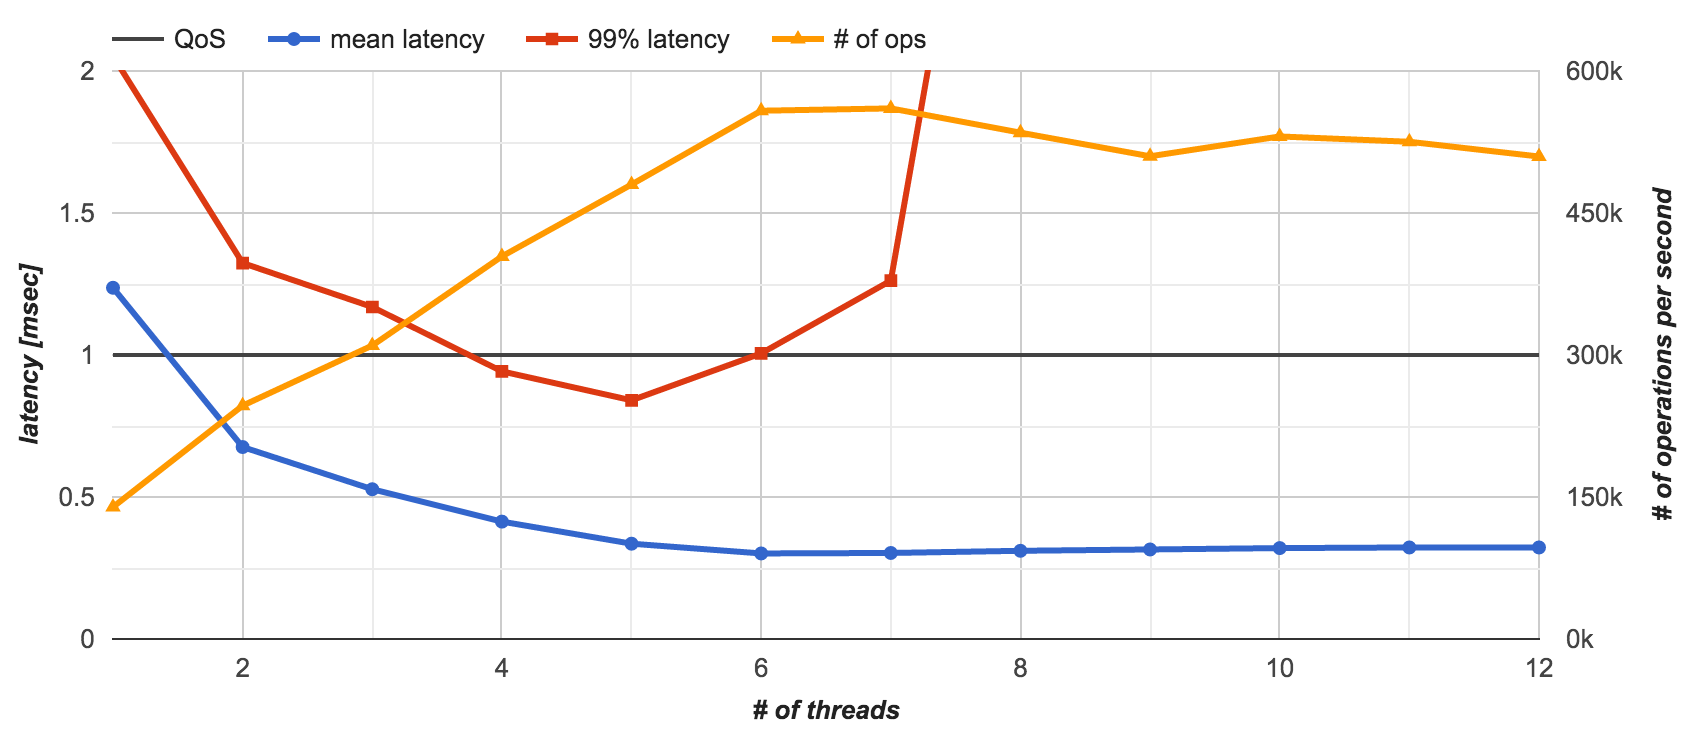
\includegraphics[width=\textwidth]{./res2/m_threads_latency.png}
    \caption{Memcached Threads: Latency \& Throughput vs Number of Threads}
    \label{fig:m_threads_latency.png}
\end{figure}

Firstly, mean latency (\textit{blue}) decreases as the number of threads increases from 1 to 6 where it reaches a minimum of 0.301ms. As the numbr of threads grows beyond 6, the mean latency increases at a slow pace.

Secondly, 99th percentile latency (\textit{red}) starts at 2.05ms, above the required QoS. As the number of threads increases, the 99th percentile latency drops sharply. With 4 to 6 threads, the 99th percentile latency satisfies the QoS with a minimum of 0.84ms reached at 5 threads. Beyond 6 threads, the 99th percentile latency rises sharply beyond the required QoS.

Thirdly, the number of operations per second (\textit{yellow}), increases linearly with the number of threads up until 6 threads where it reaches a maximum of 558k requests per second. A further increase in the number of threads results in a decrease of the number of operations per second.

Overall, QoS constraints are only achieved with 4 to 6 threads. We can attribute this effect to the multi threaded design of Memcached. With 3 threads or less, the load exerted by the clients cannot be processed quickly resulting in requests being queued up. This leads to an increased 99th percentile latency. With a sufficient number of threads to process the load effectively, a CPU core is able to service the requests sooner and therefore reduce the 99th percentile latency while also increasing the total number of operations.

With more than 6 threads, the kernel is forced to schedule multiple threads on the same core. This effect is described as `load imbalance' by Leverich \& Kozyrakis. With more than 1 Memcached thread executing on a single core, it is reasonable to expect the throughput to decrease, as opposed to only 1 Memcached thread per each core, due to context switching.

Overall, the best performance in terms of maximizing throughput and minimizing latency is provided by as many threads as CPU cores, in our case 6 threads. However, this is not in fact the minimum 99th percentile latency achieved in the benchmark - at 5 threads we obtain 99th percentile latency of 0.84ms with 480k requests per second.


\subsection{CPU Utilization}

Figure \ref{fig:m_threads_cpu} provides the \textit{mpstat} category breakdown of the CPU utilization of Memcached during the benchmark. Note that unattributed utilization accounts for idle time.

\begin{figure}[h]
    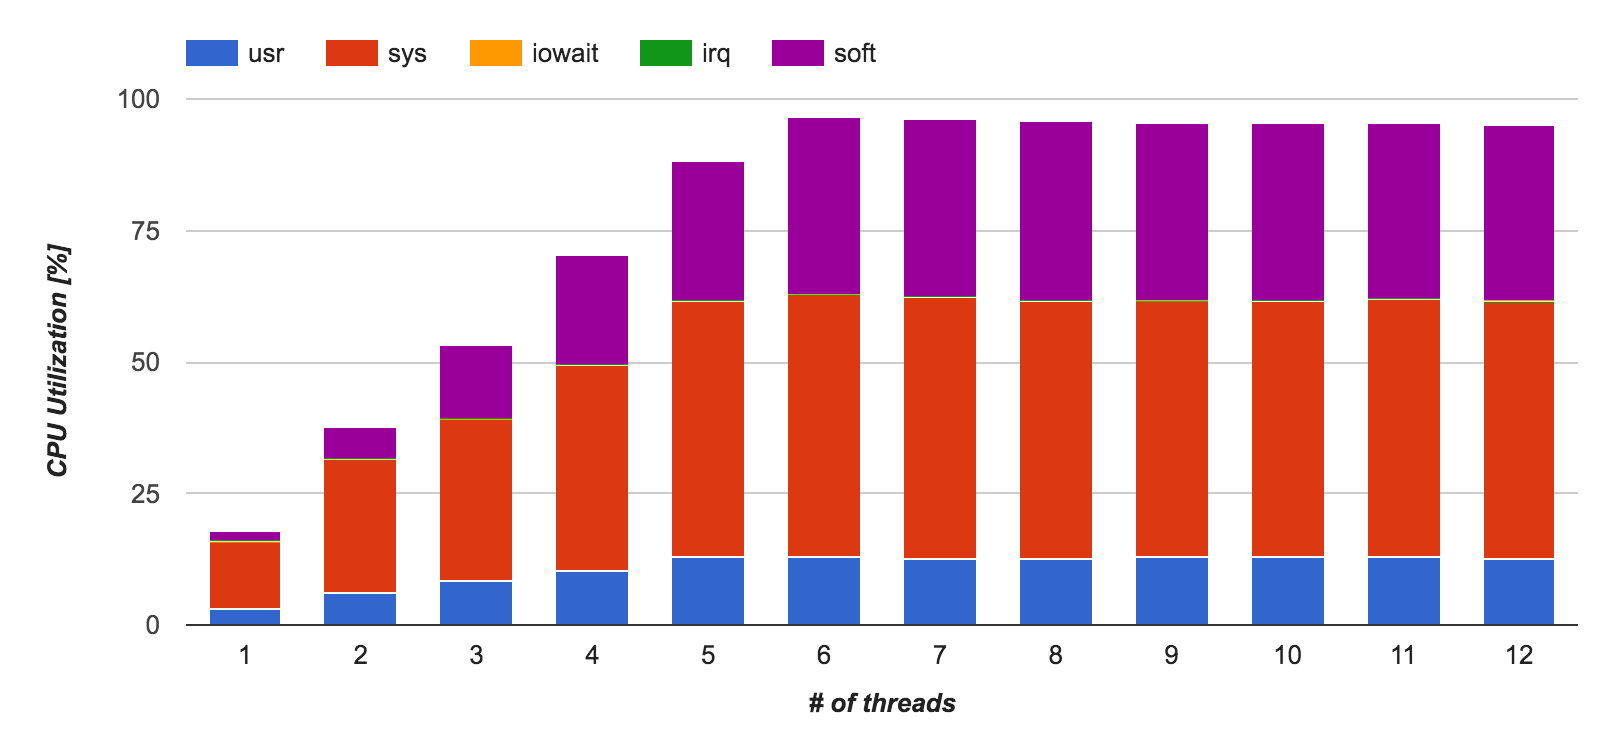
\includegraphics[width=\textwidth]{./res2/m_threads_cpu.png}
    \caption{Memcached CPU Utilization with Multiple Threads}
    \label{fig:m_threads_cpu}
\end{figure}

Firstly, Memcached CPU usage (\textit{usr}) increases linearly with the number of instances up to 6 threads and accounts for 12.7\%. With more than 6 threads, the Memcached CPU usage remains constant. This is reasonable as Memcached itself is not CPU intensive, however, a larger number of threads will require more CPU to operate effectively. Consequently, with more than 6 threads, context switching occurs due to insufficient number of CPU cores to monopolize a given core and therefore the CPU usage remains constant.

Secondly, kernel utilization increases with the number of threads up to 6 threads at which point it stabilizes and accounts for 50\%. A further increase in the number of threads does not result in increased utilization. It is reasonable to expect a large kernel CPU utilization as it is responsible for receiving and sending of network requests and memcached is a network bound application \cite{belay2014ix}.

Thirdly, similarly to kernel CPU usage, CPU utilization for software interrupts (\textit{soft}) increases with the number of threads. At 6 threads, it accounts for 33.7\%. The increase in the time spent processing software interrupts is due to overall increase in throughput as requests are processed faster. An increase in the number of requests per second directly results in an increase in the number of software interrupts received and issued by \textit{libevent}.

Finally, we observe no disk I/O wait as Memcached is an in memory object cache and therefore does not access the hard drive unless the memory is exhausted and swapping to disk is triggered. Additionally, hardware interrupt servicing \textit{irq} only accounts for 0.01\% as batching in the NIC is enabled.


\subsection{Thread Evaluation}
Increasing the number of Memcached threads results in increased throughput and decreased latency. The best performing configuration observed is with as many threads as there are CPU cores. The direct cost of increased number of threads is CPU utilization.

% ________________________________________________________

\section{Thread pinning}
\label{sec:thread-pinning}
Thread pinning is the process of assigning a \textit{set\_irq\_affinity} to each individual thread. As suggested by Leverich and Kozyrakis, "pinning memcached threads to distinct cores greatly improves load balance, consequently improving tail latency." \cite{leverich2014reconciling} and therefore the reasonable next step in optimizing memcached performance is to attempt thread pinning and analyse the results obtained.

By default, when a new process is started, its affinity is set to all available CPUs. We can discover the affinity of a given process through the following command where \textit{pid} is the process identifier.

\begin{lstlisting}
    taskset -p <pid>
\end{lstlisting}


"A Memcache instance started with n threads will spawn n + 1 threads of which the first n are worker threads and the last is a maintenance thread used for hash table expansion under high load factor." \cite{solarflarememcached}. We can discover memcached threads used for request processing using the following command where \textit{tid} is the thread id discovered previously \cite{solarflarememcached}.
\begin{lstlisting}
    ps -p <memcache-pid> -o tid= -L | sort -n | tail -n +2 | head -n -1
\end{lstlisting}

For this benchmark, the previous configuration with 6 threads will be used.

\subsection{Latency \& Throughput vs Threads}

Figure \ref{fig:m_pinning_latency} presents a comparison of Memcached with pinned threads against unpinned threads.

\begin{figure}[h]
    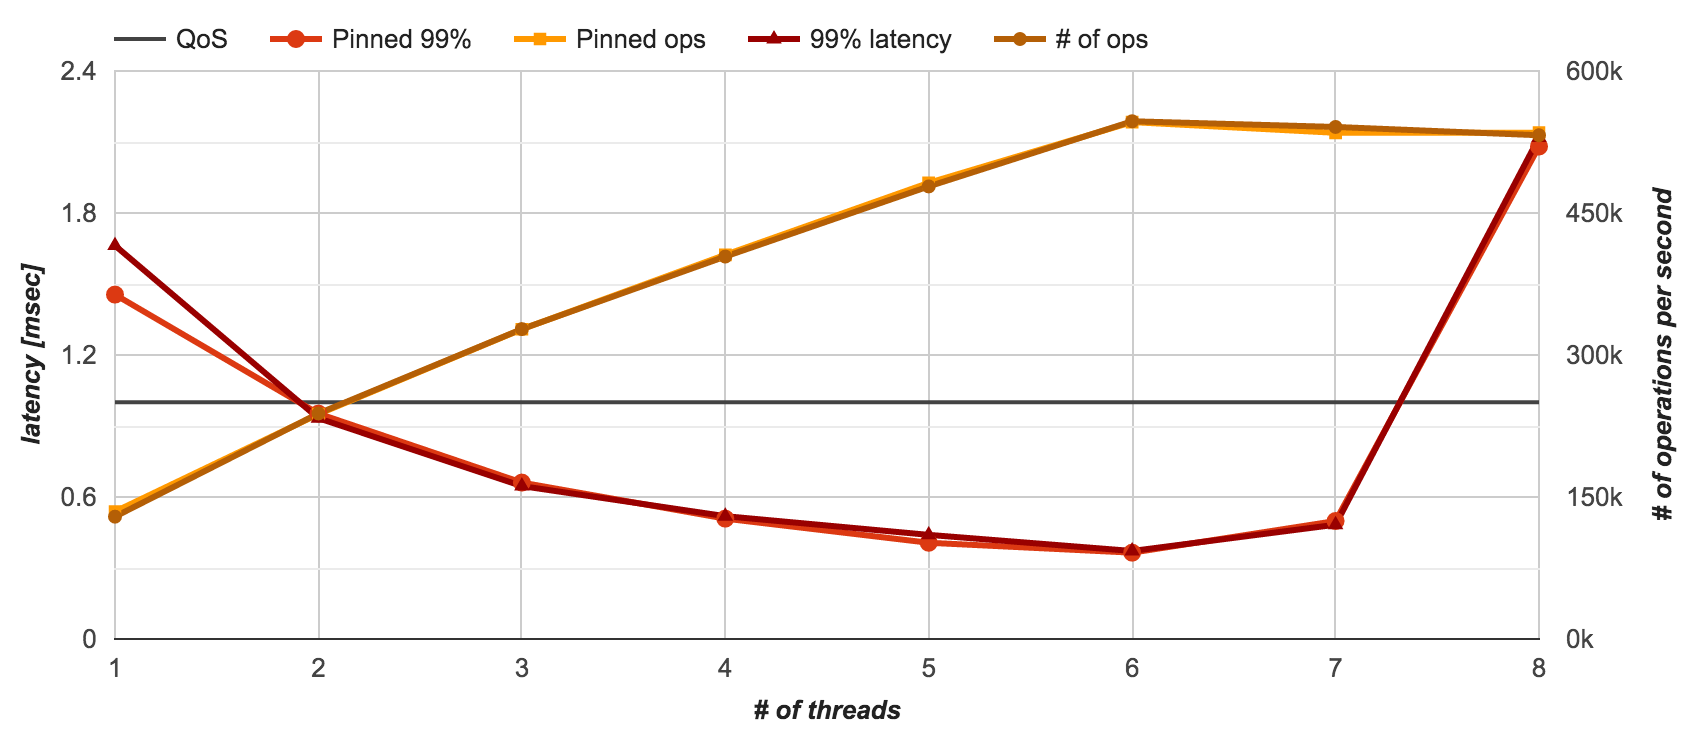
\includegraphics[width=\textwidth]{./res2/m_pinning_latency.png}
    \caption{Memcached Latency \& Throughput vs Threads: Comparison of pinned threads (labeled: \textit{Pin}) vs unpinned threads}
    \label{fig:m_pinning_latency}
\end{figure}

Overall, we can observe that there is very little change in all of the results observed. Mean latency remains the same, 99th percentile latency only differs slightly in it's minimum value at 5 threads and the number of operations per second remains the same. Overall, we find that in our benchmarks thread pinning does not affect performance significantly. This is contrary to results reported by Leverich and Kozyrakis \cite{leverich2014reconciling}. According to their research, thread pinning results in improved load balance and a result decreases 99th percentile latency. This in turn results in increased throughput.

\subsection{CPU Utilization}

Figure \ref{fig:m_pinning_cpu} presents the CPU Usage with Memcached threads pinned.

\begin{figure}[h]
    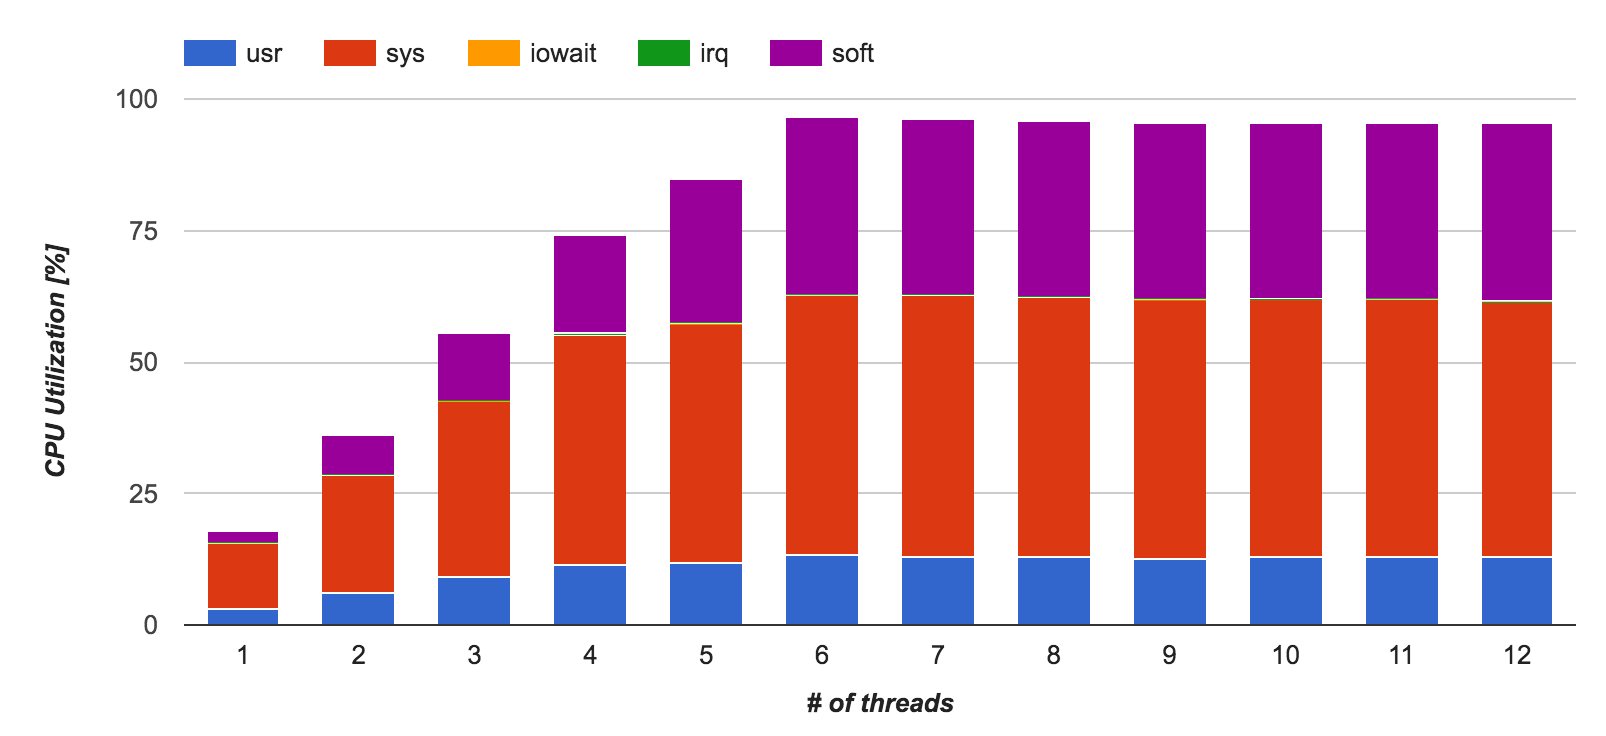
\includegraphics[width=\textwidth]{./res2/m_pinning_cpu.png}
    \caption{Pinned Memcached CPU Utilization}
    \label{fig:m_pinning_cpu}
\end{figure}

The CPU Utilization of pinned threads is nearly identical to unpinned threads presented in Figure \ref{fig:m_threads_cpu}.

\subsection{Thread Pinning Conclusion}

In our benchmarks, we have not been able to achieve the significant improvements in both latency and throughput suggested to be gained by thread pinning. This is likely due to differences in hardware as Leverich and Kozyrakis \cite{leverich2014reconciling} perform benchmarks on a significantly more performant hardware as well as running on a slightly older version of memcached.

% ________________________________________________________

\section{Group Size}
Memcached provides a configuration option \textit{-R} to set the group size used inside memcached. The group size defines the ``maximum number of requests per event, limits the number of requests processed for a given connection to prevent starvation (default: 20)'' \cite{interactive2006memcached}. This in effect means the number of requests that will be processed from a single connection before memcached switches to a different connection to enforce a fairness policy.

In this benchmark, we consider the 6-threaded Memcached configuration without thread pinning with the addition of the \textit{-R} configuration parameter to set the group size. Memcached implementation limits the minimum value of group size to be 20 while the maximum can be at most 320 (if set higher, memcached will override the setting) \cite{blake54does}. Therefore, we set up the benchmark to increase the group size by 20 in each consequtive iteration. The workload generated by the clients remains the same as in previous sections.

\subsection{Latency \& Throughput}

\begin{figure}[h]
    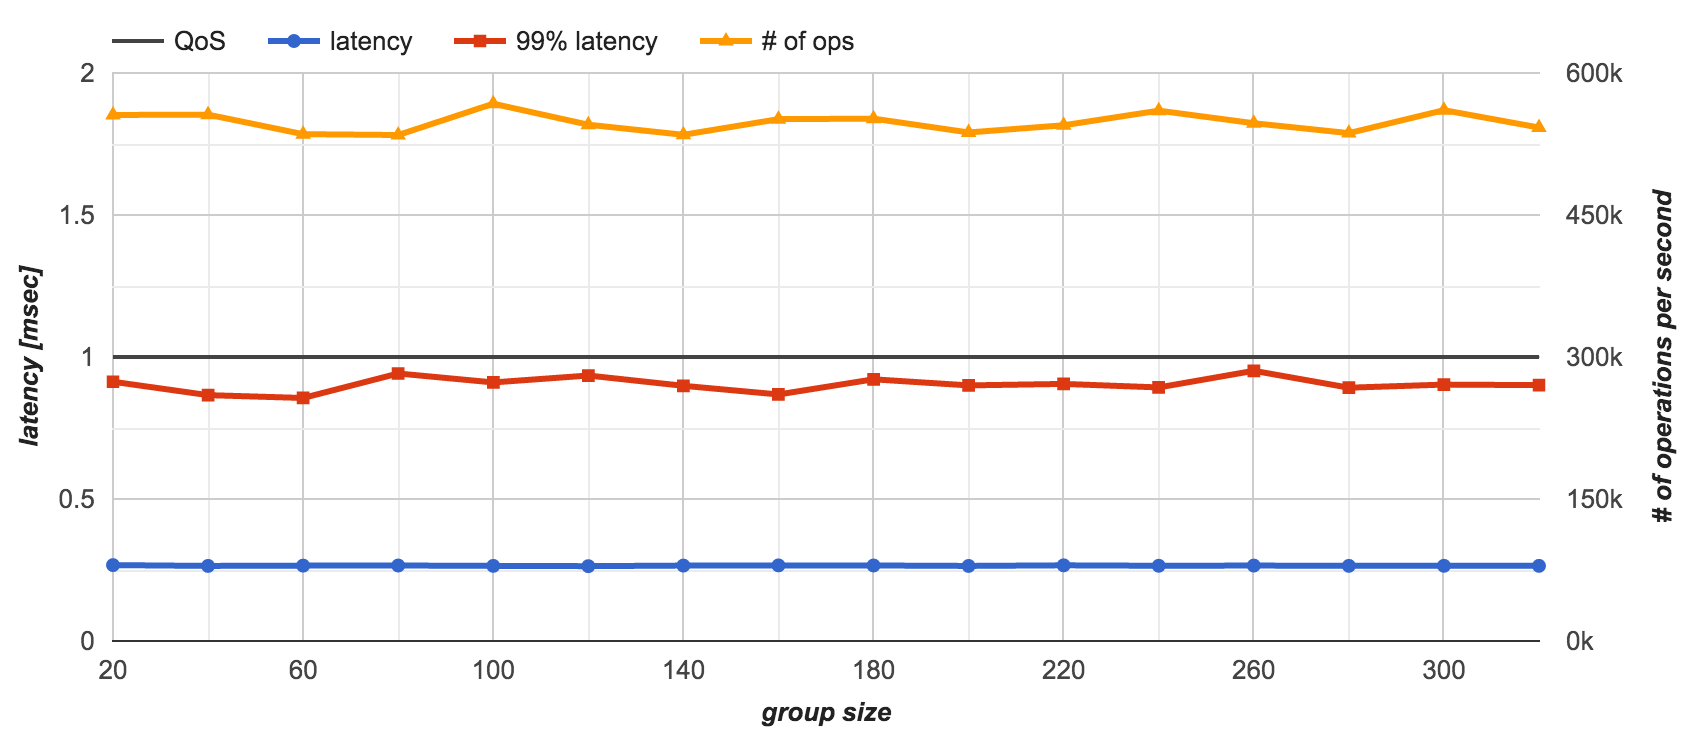
\includegraphics[width=\textwidth]{./res2/m_group_size_latency.png}
    \caption{Latency \& Throughput vs Memcached Group Size }
    \label{fig:m_group_size_latency}
\end{figure}

Figure \ref{fig:m_group_size_latency} plots the relationship between group size, latency and throughput.

Firstly, we can observe that mean latency remains unaffected as group size increases.
Secondly, the total number of operations remains stable at an average of 550k requests per second. This corresponds to the same level of throughput as observed with the default group size of 20.
Thirdly, the 99th percentile latency has decreased compared to the default at group size of 20. We have been able to reduce the 99th percentile latency to an average of 0.9ms by increasing the group size. However, there does not appear to be a strong direct correlation with a particular group size providing lower 99th percentile latency.

\subsection{CPU Utilization}

\begin{figure}[h]
    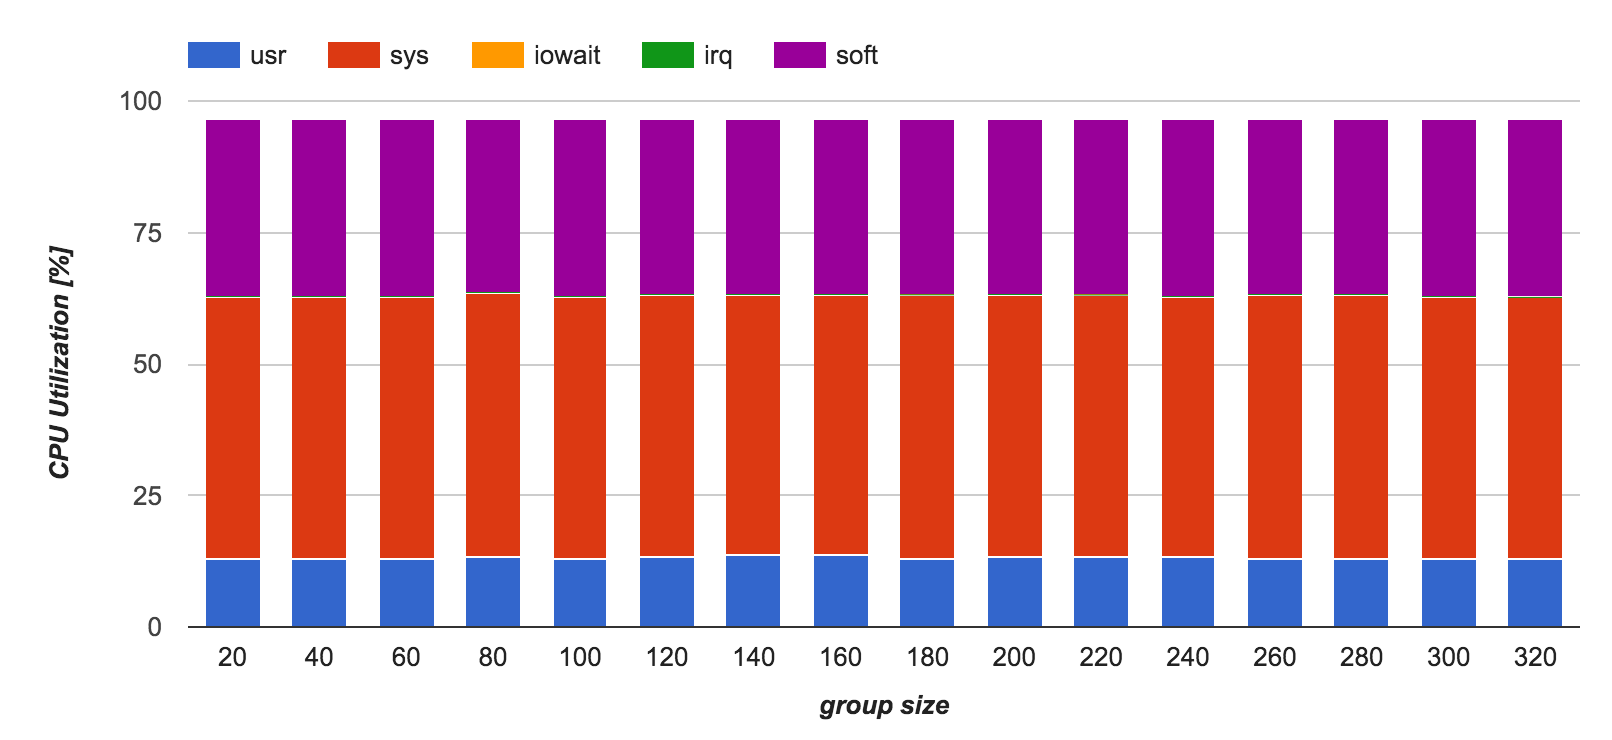
\includegraphics[width=\textwidth]{./res2/m_group_size_cpu.png}
    \caption{CPU Utilization vs Memcached Group Size}
    \label{fig:m_group_size_cpu}
\end{figure}

Figure \ref{fig:m_group_size_cpu} plots the CPU utilization reported by \textit{mpstat}. We can observe that group size does not have any impact on the distribution of CPU utilization, nor does it impact the total utilization of the CPU.

\subsection{Group Size Conclusion}

In our scenario, we have used 168 simultaneous connections from clients. In order to exploit the group size effectively, a small number of connections with very high number of requests per second may be required in order to effectively utilize the larger group size. With the hardware setup in this paper, we are unable to generate such a load and verify this claim. However, Blake and Saidi \cite{blake54does} have suggested that increasing the group size leads to increased throughput and decreased 99th percentile latency.


\section{Receive \& Transmit Queues fixing}
TODO: Haven't been able to obtain any improvements in terms of performance (both throughput and latency), not sure if the topic should still be discussed in detail.


\section{Multiple Memcached Processes}

In this section, we will examine the impact multiple memcached processed have on the overall performance of the caches as a whole. In some applications, it is important to be able to partition the system in such a way systems interact with different instances of memcached. Additionally, this information will also serve as a useful benchmark comparison for Redis performance.